%%%
% Plantilla de Memoria
% Modificación de una plantilla de Latex de Nicolas Diaz para adaptarla 
% al castellano y a las necesidades de escribir informática y matemáticas.
%
% Editada por: Mario Román
%
% License:
% CC BY-NC-SA 3.0 (http://creativecommons.org/licenses/by-nc-sa/3.0/)
%%%

%%%%%%%%%%%%%%%%%%%%%%%%%%%%%%%%%%%%%%%%%
% Thin Sectioned Essay
% LaTeX Template
% Version 1.0 (3/8/13)
%
% This template has been downloaded from:
% http://www.LaTeXTemplates.com
%
% Original Author:
% Nicolas Diaz (nsdiaz@uc.cl) with extensive modifications by:
% Vel (vel@latextemplates.com)
%
% License:
% CC BY-NC-SA 3.0 (http://creativecommons.org/licenses/by-nc-sa/3.0/)
%
%%%%%%%%%%%%%%%%%%%%%%%%%%%%%%%%%%%%%%%%%

%----------------------------------------------------------------------------------------
%	PAQUETES Y CONFIGURACIÓN DEL DOCUMENTO
%----------------------------------------------------------------------------------------

%%% Configuración del papel.
% microtype: Tipografía.
% mathpazo: Usa la fuente Palatino.
\documentclass[a4paper, 20pt]{article}
\usepackage[a4paper,margin=1in]{geometry}
\usepackage[protrusion=true,expansion=true]{microtype}
\usepackage{mathpazo}

% Indentación de párrafos para Palatino
\setlength{\parindent}{0pt}
  \parskip=8pt
\linespread{1.05} % Change line spacing here, Palatino benefits from a slight increase by default


%%% Castellano.
% noquoting: Permite uso de comillas no españolas.
% lcroman: Permite la enumeración con numerales romanos en minúscula.
% fontenc: Usa la fuente completa para que pueda copiarse correctamente del pdf.
\usepackage[spanish,es-noquoting,es-lcroman,es-tabla,,es-nodecimaldot]{babel}
\usepackage[utf8]{inputenc}
\usepackage{fontenc}
\selectlanguage{spanish}

%%% Matemáticas
\usepackage{amsmath}

%%% Gráficos
\usepackage{graphicx} % Required for including pictures
\usepackage{wrapfig} % Allows in-line images
\graphicspath{{./fig/}}
\usepackage[usexcolor=false, inkscape=true]{svg} % Required for including svg
\svgpath{{./fig/}}
\usepackage[usenames,dvipsnames]{color} % Coloring code



%%% Pseudocódigo
\usepackage{algorithmicx}
\usepackage[ruled]{algorithm}
\usepackage{algpseudocode}

\newcommand{\alg}{\texttt{algorithmicx}}
\newcommand{\old}{\texttt{algorithmic}}
\newcommand{\euk}{Euclid}
\newcommand\ASTART{\bigskip\noindent\begin{minipage}[b]{0.5\linewidth}}
\newcommand\ACONTINUE{\end{minipage}\begin{minipage}[b]{0.5\linewidth}}
\newcommand\AENDSKIP{\end{minipage}\bigskip}
\newcommand\AEND{\end{minipage}}

%%% Código
\usepackage{listings}

%%% Tablas
\usepackage{tabularx}
\usepackage{float}
\usepackage{longtable}
\usepackage{adjustbox}
\usepackage{booktabs}
\usepackage{array}
\newcolumntype{L}[1]{>{\raggedright\let\newline\\\arraybackslash\hspace{0pt}}m{#1}}
\newcolumntype{C}[1]{>{\centering\let\newline\\\arraybackslash\hspace{0pt}}m{#1}}
\newcolumntype{R}[1]{>{\raggedleft\let\newline\\\arraybackslash\hspace{0pt}}m{#1}}

% Enlaces y colores
\usepackage{hyperref}
\usepackage[dvipsnames]{xcolor}
\definecolor{webgreen}{rgb}{0,0.5,0}
\hypersetup{
  colorlinks=true,
  citecolor=RoyalBlue,
  urlcolor=RoyalBlue,
  linkcolor=RoyalBlue
}

%%% Bibliografía
\usepackage[backend=biber]{biblatex}
\DefineBibliographyStrings{spanish}{
  urlseen = {Último acceso}
}
\addbibresource{IN-P2.bib}

%----------------------------------------------------------------------------------------
%	TÍTULO
%----------------------------------------------------------------------------------------
% Configuraciones para el título.
% El título no debe editarse aquí.
\renewcommand{\maketitle}{
  \begin{flushright} % Right align
  
  {\LARGE\@title} % Increase the font size of the title
  
  \vspace{50pt} % Some vertical space between the title and author name
  
  {\large\@author} % Author name
  \\\@date % Date
  \vspace{40pt} % Some vertical space between the author block and abstract
  \end{flushright}
}

%% Título
\title{\textbf{Título}\\ % Title
Subtítulo} % Subtitle

\author{\textsc{Autor1,\\Autor2} % Author
\\{\textit{Universidad de Granada}}} % Institution

\date{\today} % Date

%-----------------------------------------------------------------------------------------
%	DOCUMENTO
%-----------------------------------------------------------------------------------------

\begin{document}

%-----------------------------------------------------------------------------------------
%	TITLE PAGE
%-----------------------------------------------------------------------------------------

\begin{titlepage} % Suppresses displaying the page number on the title page and the subsequent page counts as page 1
	
	\raggedleft % Right align the title page
	
	\rule{1pt}{\textheight} % Vertical line
	\hspace{0.05\textwidth} % Whitespace between the vertical line and title page text
	\parbox[b]{0.8\textwidth}{ % Paragraph box for holding the title page text, adjust the width to move the title page left or right on the page
		
		{\Huge\bfseries Práctica 3:\\[0.5\baselineskip] Competición en DrivenData}\\[2\baselineskip] % Title
		{\large\textit{Curso 2019/2020}}\\[4\baselineskip] % Subtitle or further description
		{\Large\textsc{Sofía Almeida Bruno}\\[0.5\baselineskip]sofialmeida@correo.ugr.es} % Author name, lower case for consistent small caps
		
		\vspace{0.4\textheight} % Whitespace between the title block and the publisher
		
		{\noindent Grupo IN 2\\[0.5\baselineskip] Jueves 9:30-10:30}\\[\baselineskip] % Publisher and logo
	}

\end{titlepage}

%% Resumen (Descomentar para usarlo)
%\renewcommand{\abstractname}{Resumen} % Uncomment to change the name of the abstract to something else
%\begin{abstract}
% Resumen aquí
%\end{abstract}

%% Palabras clave
%\hspace*{3,6mm}\textit{Keywords:} lorem , ipsum , dolor , sit amet , lectus % Keywords
%\vspace{30pt} % Some vertical space between the abstract and first section


%% Índice
{\parskip=2pt
  \tableofcontents
}
\pagebreak

%%% Inicio del documento
%%%%%%%%%%%%%%%%%%%%%%%%%%%%%%%%%%%%%%%%%%%%%%%%%%%%%%%%%%%%%%%%%%%
%       DESCRIPCIÓN DEL PROBLEMA
%%%%%%%%%%%%%%%%%%%%%%%%%%%%%%%%%%%%%%%%%%%%%%%%%%%%%%%%%%%%%%%%%%%
%\section{Introducción} TODO ?


%%%%%%%%%%%%%%%%%%%%%%%%%%%%%%%%%%%%%%%%%%%%%%%%%%%%%%%%%%%%%%%%%%%
%       Captura de pantalla de Submissions
%%%%%%%%%%%%%%%%%%%%%%%%%%%%%%%%%%%%%%%%%%%%%%%%%%%%%%%%%%%%%%%%%%%
\section{Captura de pantalla de Submissions}
\label{sec:subsimissions}
\pagebreak


%%% Inicio del documento
%%%%%%%%%%%%%%%%%%%%%%%%%%%%%%%%%%%%%%%%%%%%%%%%%%%%%%%%%%%%%%%%%%%
%       Pruebas realizadas
%%%%%%%%%%%%%%%%%%%%%%%%%%%%%%%%%%%%%%%%%%%%%%%%%%%%%%%%%%%%%%%%%%%
\section{Pruebas realizadas}
\begin{table}[H]
\centering
\caption{Pruebas realizadas}
\label{tab:pruebas}
\makebox[\textwidth][c]{\begin{tabular}{lL{2cm}lllL{3cm}L{2.5cm}L{3.5cm}}
\toprule
ID & Fecha-hora & Pos. & Sc.-Training & Sc.-Test & Preprocesado & Algoritmos & Parámetros\\
\midrule
00 & 5/12/2019 10:07:58 UTC & 315 & 0.7264 & 0.6883 & - & Lightgbm & {\ttfamily objective = 'regression\_l1', n\_estimators = 200, n\_jobs = 2}\\

01 & 19/12/2019 11:18:10 UTC & 356 & 0.7358 & 0.6874 & - & Lightgbm & {\ttfamily objective = 'regression\_l1', n\_estimators = 200, n\_jobs = 2, feature\_fraction = 0.5, learning\_rate = 0.1, num\_leaves = 50}\\

02 & 22/12/2019 17:32:55 UTC & 360 & 0.7294 & 0.6894 & - & Lightgbm & {\ttfamily objective = 'regression\_l1', n\_estimators = 200, n\_jobs = 2, num\_leaves = 35, scale\_pos\_weight = 0.1}\\

03 & 22/12/2019 20:39:08 UTC & 243 & 0.7339 & 0.7227 & \texttt{get\_dummies} para todas las variables categóricas & Lightgbm & {\ttfamily objective='regression\_l1', n\_estimators=200, n\_jobs=2, num\_leaves = 40, scale\_pos\_weight = 0.1}\\

04 & 23/12/2019 17:14:45 UTC & 242 & 0.7342 & 0.7245 & \texttt{get\_dummies} para todas las variables categóricas. Selección de variables con \texttt{VarianceThreshold}, umbral 0.95 & Lightgbm & {\ttfamily objective='regression\_l1', n\_estimators=200, n\_jobs=2, num\_leaves = 40, scale\_pos\_weight = 0.1}\\

05 & 23/12/2019 18:58:58 UTC & 242 & 0.7335 & 0.7228 & \texttt{get\_dummies} para todas las variables categóricas. Selección de variables con \texttt{SelectKBest}, $k =35$ & Lightgbm & {\ttfamily objective='regression\_l1', n\_estimators=200, n\_jobs=2, num\_leaves = 40, scale\_pos\_weight = 0.1}\\

06 & 23/12/2019 21:29:30 UTC & 234 & 0.7375 & 0.7253 & \texttt{get\_dummies} para todas las variables categóricas. Selección de variables con \texttt{VarianceThreshold}, umbral 0.95 & Lightgbm & {\ttfamily objective = 'regression\_l1', n\_estimators=200, n\_jobs=2, num\_leaves = 45, scale\_pos\_weight = 0.1}\\
\bottomrule
\end{tabular}}
\end{table}
\newpage

\section{Diario de pruebas}
\subsection{\texttt{p3\_00}}
Comenzamos aprendiendo a subir los resultados de test a la plataforma para que puedan ser validados. El script utilizado en esta ocasión es el proporcionado por el profesor de la asignatura. No se realiza ningún preprocesado y el algoritmo a utilizar es Lightgbm un algoritmo de boosting.
%TODO: Comentar algo de lightgbm vs xgboost

\subsection{\texttt{p3\_01}}
\subsubsection{Análisis exploratorio de los datos}

Antes de decidir qué hacer a continuación debemos conocer cierta información sobre los datos. Podemos pensar que necesitamos algún tipo de preprocesado, pues es lo habitual en este tipo de problema, pero sin conocer exactamente cómo son nuestros datos, si tienen o no ruido, la cantidad de valores perdidos, correlación entre las variables, \dots no podremos decidir cómo enfocar el preprocesado ni qué necesidades tiene el conjunto. Para ello comenzamos a escribir algunas funciones de visualización que nos permitan conocer esta información, se encuentran en el \textit{script} \texttt{visualization.py}

Inspirándonos en 
https://www.kaggle.com/kerneler/starter-richter-s-predictor-modeling-e7f51e9e-e
observamos en la Figura \ref{fig:tam_clases} la distribución de las clases.

\begin{figure}[H]
    \centering
    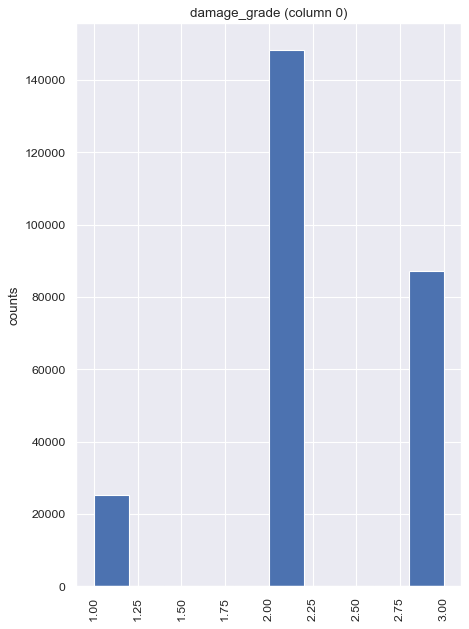
\includegraphics[height=0.6\textwidth, width=0.6\textwidth]{260601_dist}
    \caption{Tamaño de las clases}
    \label{fig:tam_clases}
\end{figure}

Nuestras clases están claramente desbalanceadas, en la Tabla \ref{tab:tam_clas} observamos con exactitud el número de ejemplos que tenemos de cada clase. Ante esta situación se nos ocurren dos opciones: elegir un algoritmo que esté diseñado para manejar esta situación, utilizar técnicas específicas para paliarlo.

% Tabla tamaño de clases
\begin{table}[H]
\centering
\caption{Tamaño de las clases}
\label{tab:tam_clas}
\begin{tabular}{lrr}
\toprule
Clase & Número de elementos & Tamaño de la clase\\
\midrule
1 & 25124 & 9.64\%\\
2 & 148259 & 56.89\%\\
3 & 87218 & 33.47\%\\
\bottomrule
\end{tabular}
\end{table}

También podemos observar la correlación entre las variables en la Figura \ref{fig:corr_matrix}.


\begin{figure}[H]
  \centering
  \includesvg[height=1\textwidth, width=1\textwidth]{corr_matrix}
  \caption{Matriz de correlación}
  \label{fig:corr_matrix}
\end{figure}


% A partir de aquí la inspiración viene de...
% https://www.kaggle.com/jaylaksh94/model-for-nepal-earthquake-damage
Mediante \texttt{data\_x.info()} conocemos que de las 38 variables 30 son numéricas y 8 categóricas, accedemos a la descripción del problema en %https://www.drivendata.org/competitions/57/nepal-earthquake/page/136/
para conocer cuántos posibles valores toman las variables categóricas. Toman entre 3 y 10 posibles valores. En esta página también nos percatamos de que, de las variables numéricas, muchas son de tipo binario.

Ejecutando \texttt{data\_x.isnull().any()} nos damos cuenta de que nuestras variables no contienen valores perdidos, podemos ahorrarnos la imputación de valores perdidos.

% TODO: Ver si hay ruido

\subsubsection{Ajuste de Lightgbm}

Para tratar de conseguir mejores resultados tenemos, a priori, dos caminos: preprocesar los datos, mejorar el algoritmo. Para mejorar el algoritmo hay, a su vez, dos opciones: elegir el algoritmo y ajustar sus parámetros.

En primer lugar trataremos de ajustar los parámetros de Lightgbm a ver si mejora el resultado. Usando el código de ejemplo \texttt{ejemplo\_ds\_avanzado} nos centraremos en los parámetros \texttt{feature\_fraction} (que tomará ..., \texttt{learning\_rate}, \texttt{num\_leaves}. Fijando \texttt{n\_estimators = 200}. Tras realizar el \texttt{GridSearch} se obtiene (tras 10 minutos de ejecución) que los mejores parámetros son: \texttt{feature\_fraction = 0.5}, \texttt{learning\_rate = 0.1},  \texttt{n\_estimators = 200}, \texttt{num\_leaves = 50}.

Obtenemos un resultado en training de 0.7358 y en test de 0.6874, disminuyendo con respecto al anterior envío, a pesar de haber aumentado en test. ¿Se está produciendo sobre ajuste?

\subsection{\texttt{p3\_02}}

%% Comprobamos qué ocurre si nos quedamos con menor \texttt{learning\_rate}. Usamos los parámetros ajustados, modificando solo la variable comentada. Los parámetros utilizados son: \texttt{feature\_fraction = 0.5}, \texttt{learning\_rate = 0.05},  \texttt{n\_estimators = 200}, \texttt{num\_leaves = 50}.
Nos preguntamos qué está provocando este sobreajuste, así comprobamos los valores de las variables por defecto y los utilizados. El que más se diferencia es \texttt{num\_leaves}, por defecto es 31 y estamos tomando 50. Es complicado saber hasta qué punto podemos aumentar el número de hojas sin que se llegue a producir el sobre ajuste que provoca malos resultados en la fase de test, más teniendo en cuenta que el número de pruebas a realizar es limitado. Por ello, proseguiré tratando de mejorar el rendimiento de este algoritmo de otro modo.

% https://lightgbm.readthedocs.io/en/latest/Parameters.html
Para paliar el desbalanceamiento de las clases se pueden usar dos parámetros: \texttt{is\_unbalance} o \texttt{scale\_pos\_weight}.
Probaremos a configurar ambos parámetros a ver con cuál conseguimos realmente mejor resultado.

Así, en \texttt{p3\_02\_unbalance.py} partimos del código utilizado en \texttt{p3\_00.py} añadiendo las variables \texttt{num\_classes = 3} y \texttt{is\_unbalance = True}. Conseguimos exactamente el mismo resultado que en el archivo de partida (los archivos \texttt{submission} correspondientes no se diferencian) a pesar de que por defecto se asumía que no había desbalanceo. 

Probamos con la otra opción: variamos el peso de la clase positiva entre 0.1 y 0.6 modificando el parámetro \texttt{scale\_pos\_weight}.
Así, terminamos ejecutando el algoritmo con {\ttfamily n\_estimators = 200, num\_leaves = 35, scale\_pos\_weight = 0.1} que consiguió una puntuación de 0.7294 en entrenamiento y 0.6894 al realizar el envío (mejorando la mejor solución obtenida hasta el momento).

\subsection{p3\_03}
% https://stackoverflow.com/questions/24109779/running-get-dummies-on-several-dataframe-columns#24109916
% https://pandas.pydata.org/pandas-docs/stable/reference/api/pandas.get_dummies.html
Una opción que podemos utilizar para preprocesar es, en vez de convertir las variables categóricas a numéricas, realizar un \textit{one-to-many} en el que binarizamos las variables categóricas. Como observamos que eran 8 y que no tomaban demasiados valores, además de que Lightgbm es un algoritmo rápido, probamos este preprocesado. 

Pandas ofrece una función que realiza la transformación sobre el conjunto de datos, mediante la función \texttt{get\_dummies}. En el archivo \texttt{p3\_03.py} encontramos el código correspondiente a esta ejecución. Pasamos de 38 a 68 características.

Conseguimos una puntuación en test de 0.7339 y en prueba de 0.7227.

\subsection{\texttt{p3\_04}}

Aunque Lightgbm es un algoritmo ligero y se puede ejecutar con las 68 variables que conseguimos tras binarizar las categóricas, puede que no todas ellas sean importantes para clasificar si el edificio ha sido dañado o no, alejando el modelo del modelo ideal. Por ello, partiendo del código anterior en el que utlizamos Lightgbm con 0.1 para \texttt{scale\_pos\_weight} añadimos un método de selección de variables al preprocesado.

% https://scikit-learn.org/stable/modules/feature_selection.html
Nuestro primer intento consiste en eliminar las variables con varianza baja. Por defecto, elimina las variables que tengan varianza nula, esto es, aquellas variables que tengan el mismo valor para todos los ejemplos. Indicamos un umbral para que elimine. Por ejemplo, para 0.9 obtenemos de f1 score en training 0.7319 (22 variables, en torno a 15 segundos por partición). Con un umbral de 0.95 nos quedamos con 33 variables finalmente, los tiempos por partición van desde 16 hasta 20 segundos, pero la puntuación se ve favorecida (en training) siendo ahora 0.7342. La puntuación al subirlo en la web es de 0.7245 (mejorando en milésimas al programa base sin selección de variables).

Tratamos de ver la importancia de cada variable adaptando...%https://stackoverflow.com/questions/53413701/feature-importance-using-lightgbm/53578643#53578643
% https://scikit-learn.org/stable/modules/generated/sklearn.feature_selection.VarianceThreshold.html
% https://lightgbm.readthedocs.io/en/latest/pythonapi/lightgbm.LGBMClassifier.html
en la Figura \ref{fig:lgbm_imp_04} podemos ver el número de veces que una variable se usa en un modelo.
\begin{figure}[H]
    \centering
    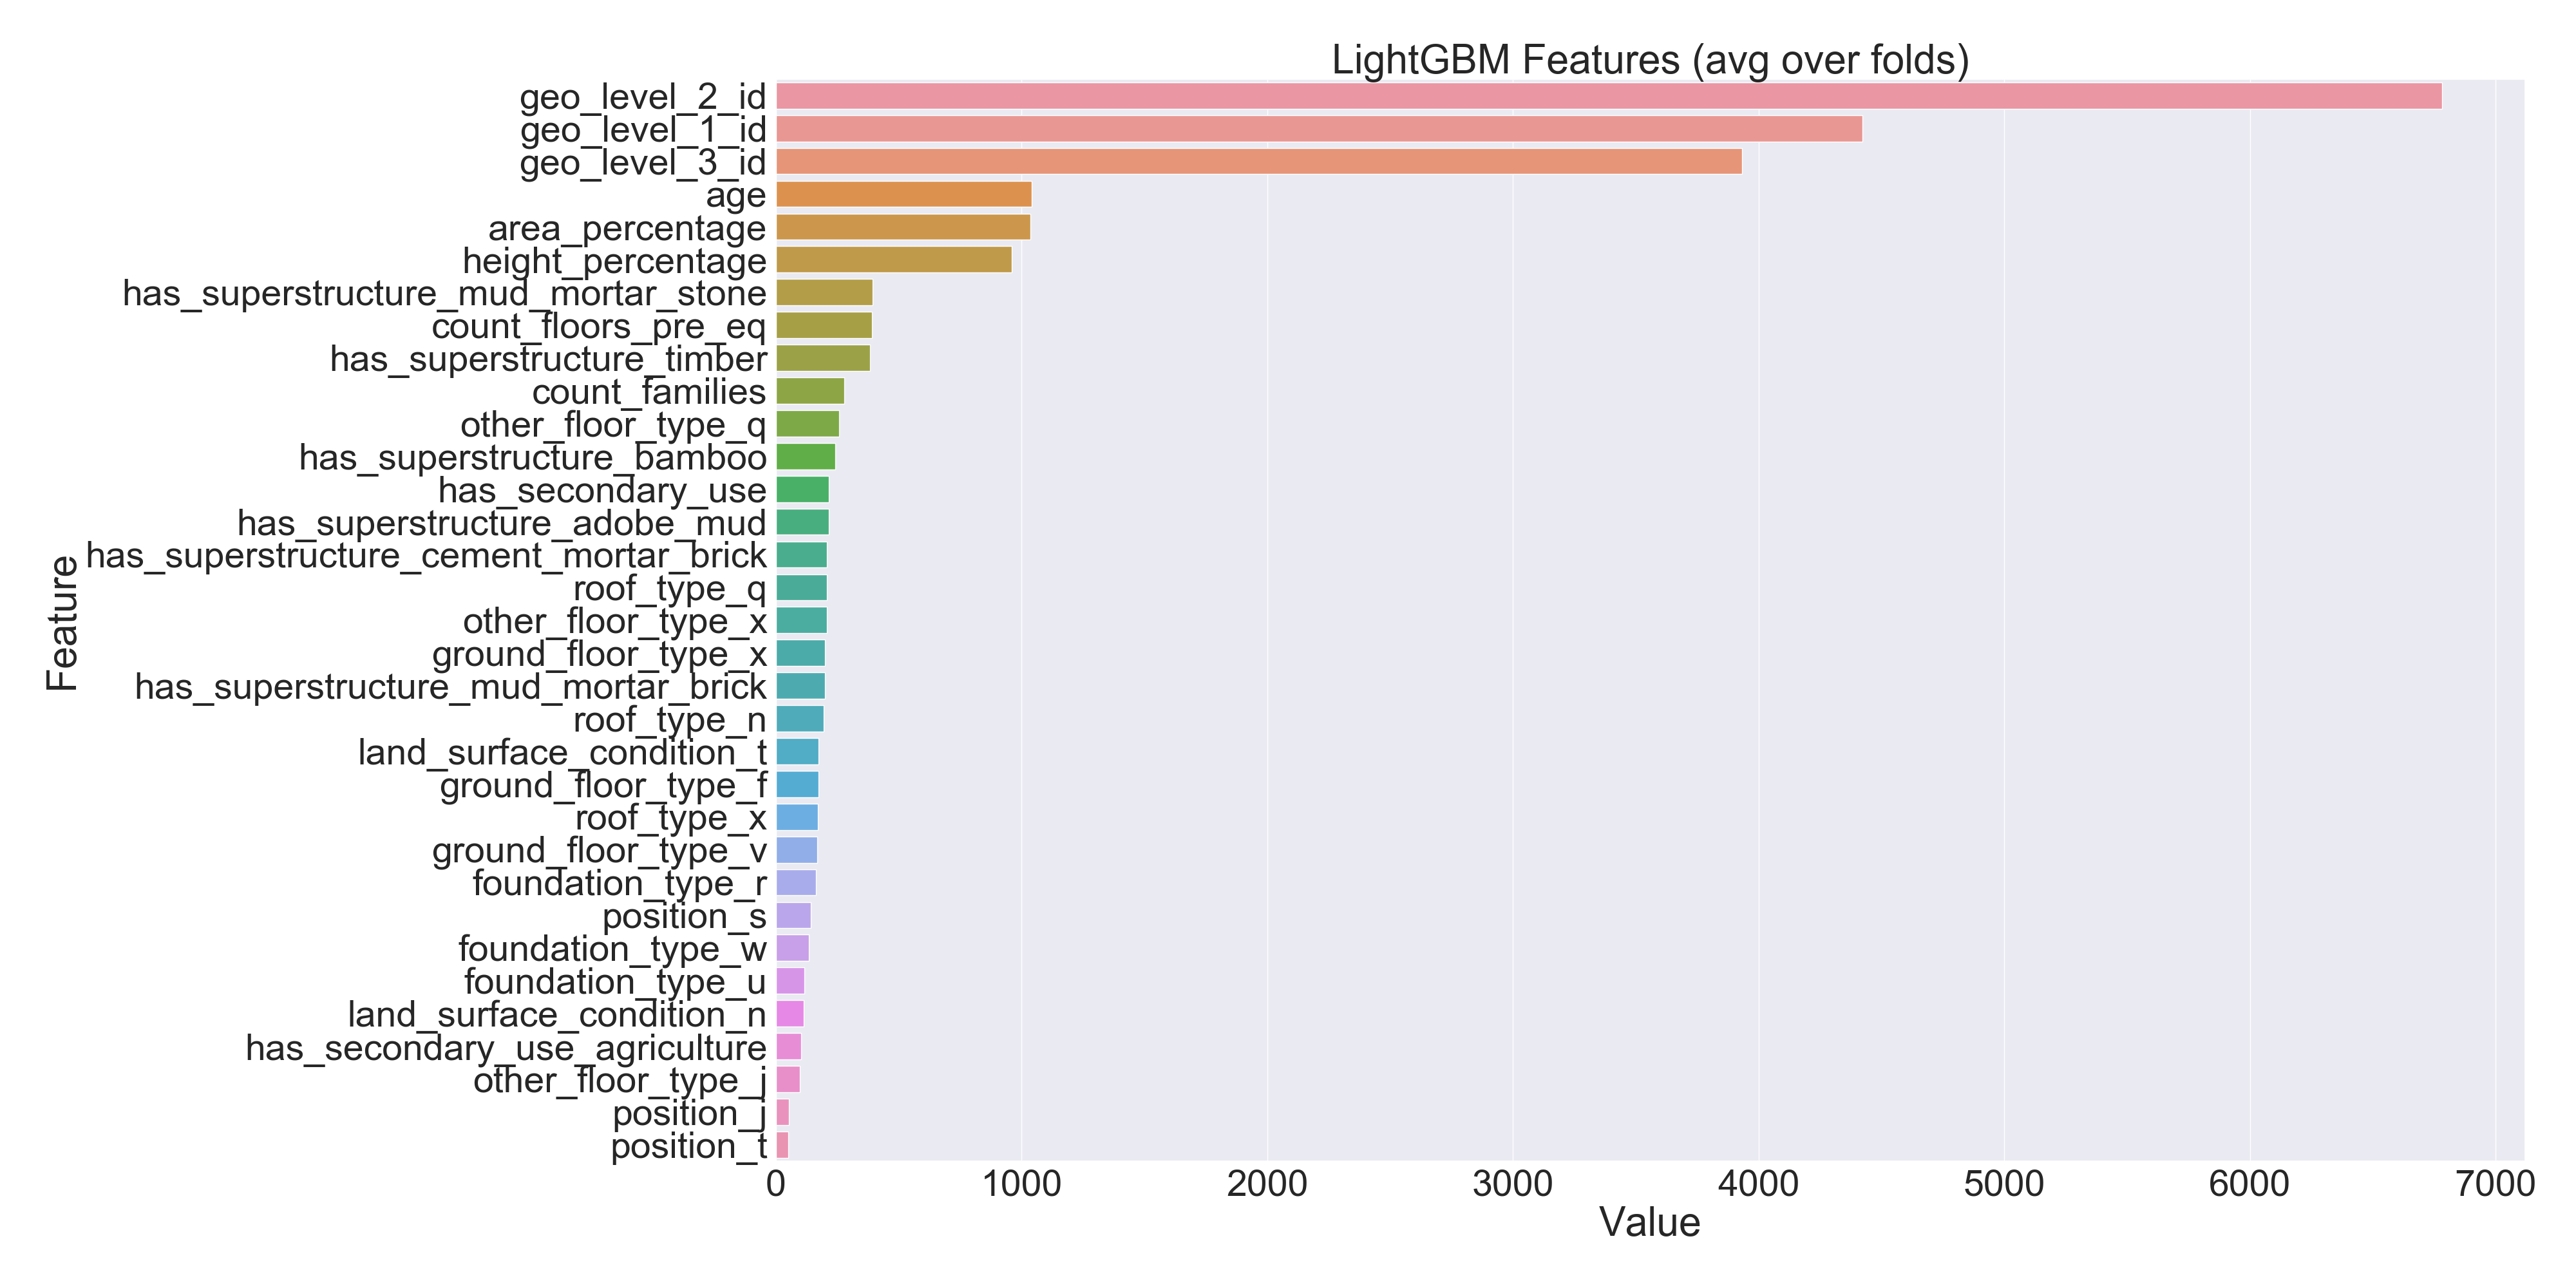
\includegraphics[height=0.9\textwidth, width=1.0\textwidth]{lgbm_importances04}
    \caption{Importancia de las variables}
    \label{fig:lgbm_imp_04}
\end{figure}

\subsection{\texttt{p3\_05}}
Seleccionando variables a partir de su varianza hemos mejorado algunas milésimas el resultado, igual utilizando algún otro método de selección más complejo logramos ajustarnos un poco mejor a las variables realmente determinantes en nuestro problema.

Probamos a seleccionar los k mejores
% https://scikit-learn.org/stable/modules/generated/sklearn.feature_selection.SelectKBest.html#sklearn.feature_selection.SelectKBest

Notamos que los tiempos de ejecución disminuyen, pasan a rondar los 10 segundos. El resultado en entrenamiento es una puntuación f1-score de 0.7251 para 10 características. Observamos en la Figura 
\label{fig:lgbm_imp_05_10} que las cuatro primeras variables son las mismas que seleccionando según la varianza, pero a partir de ahí varían.
\begin{figure}[H]
    \centering
    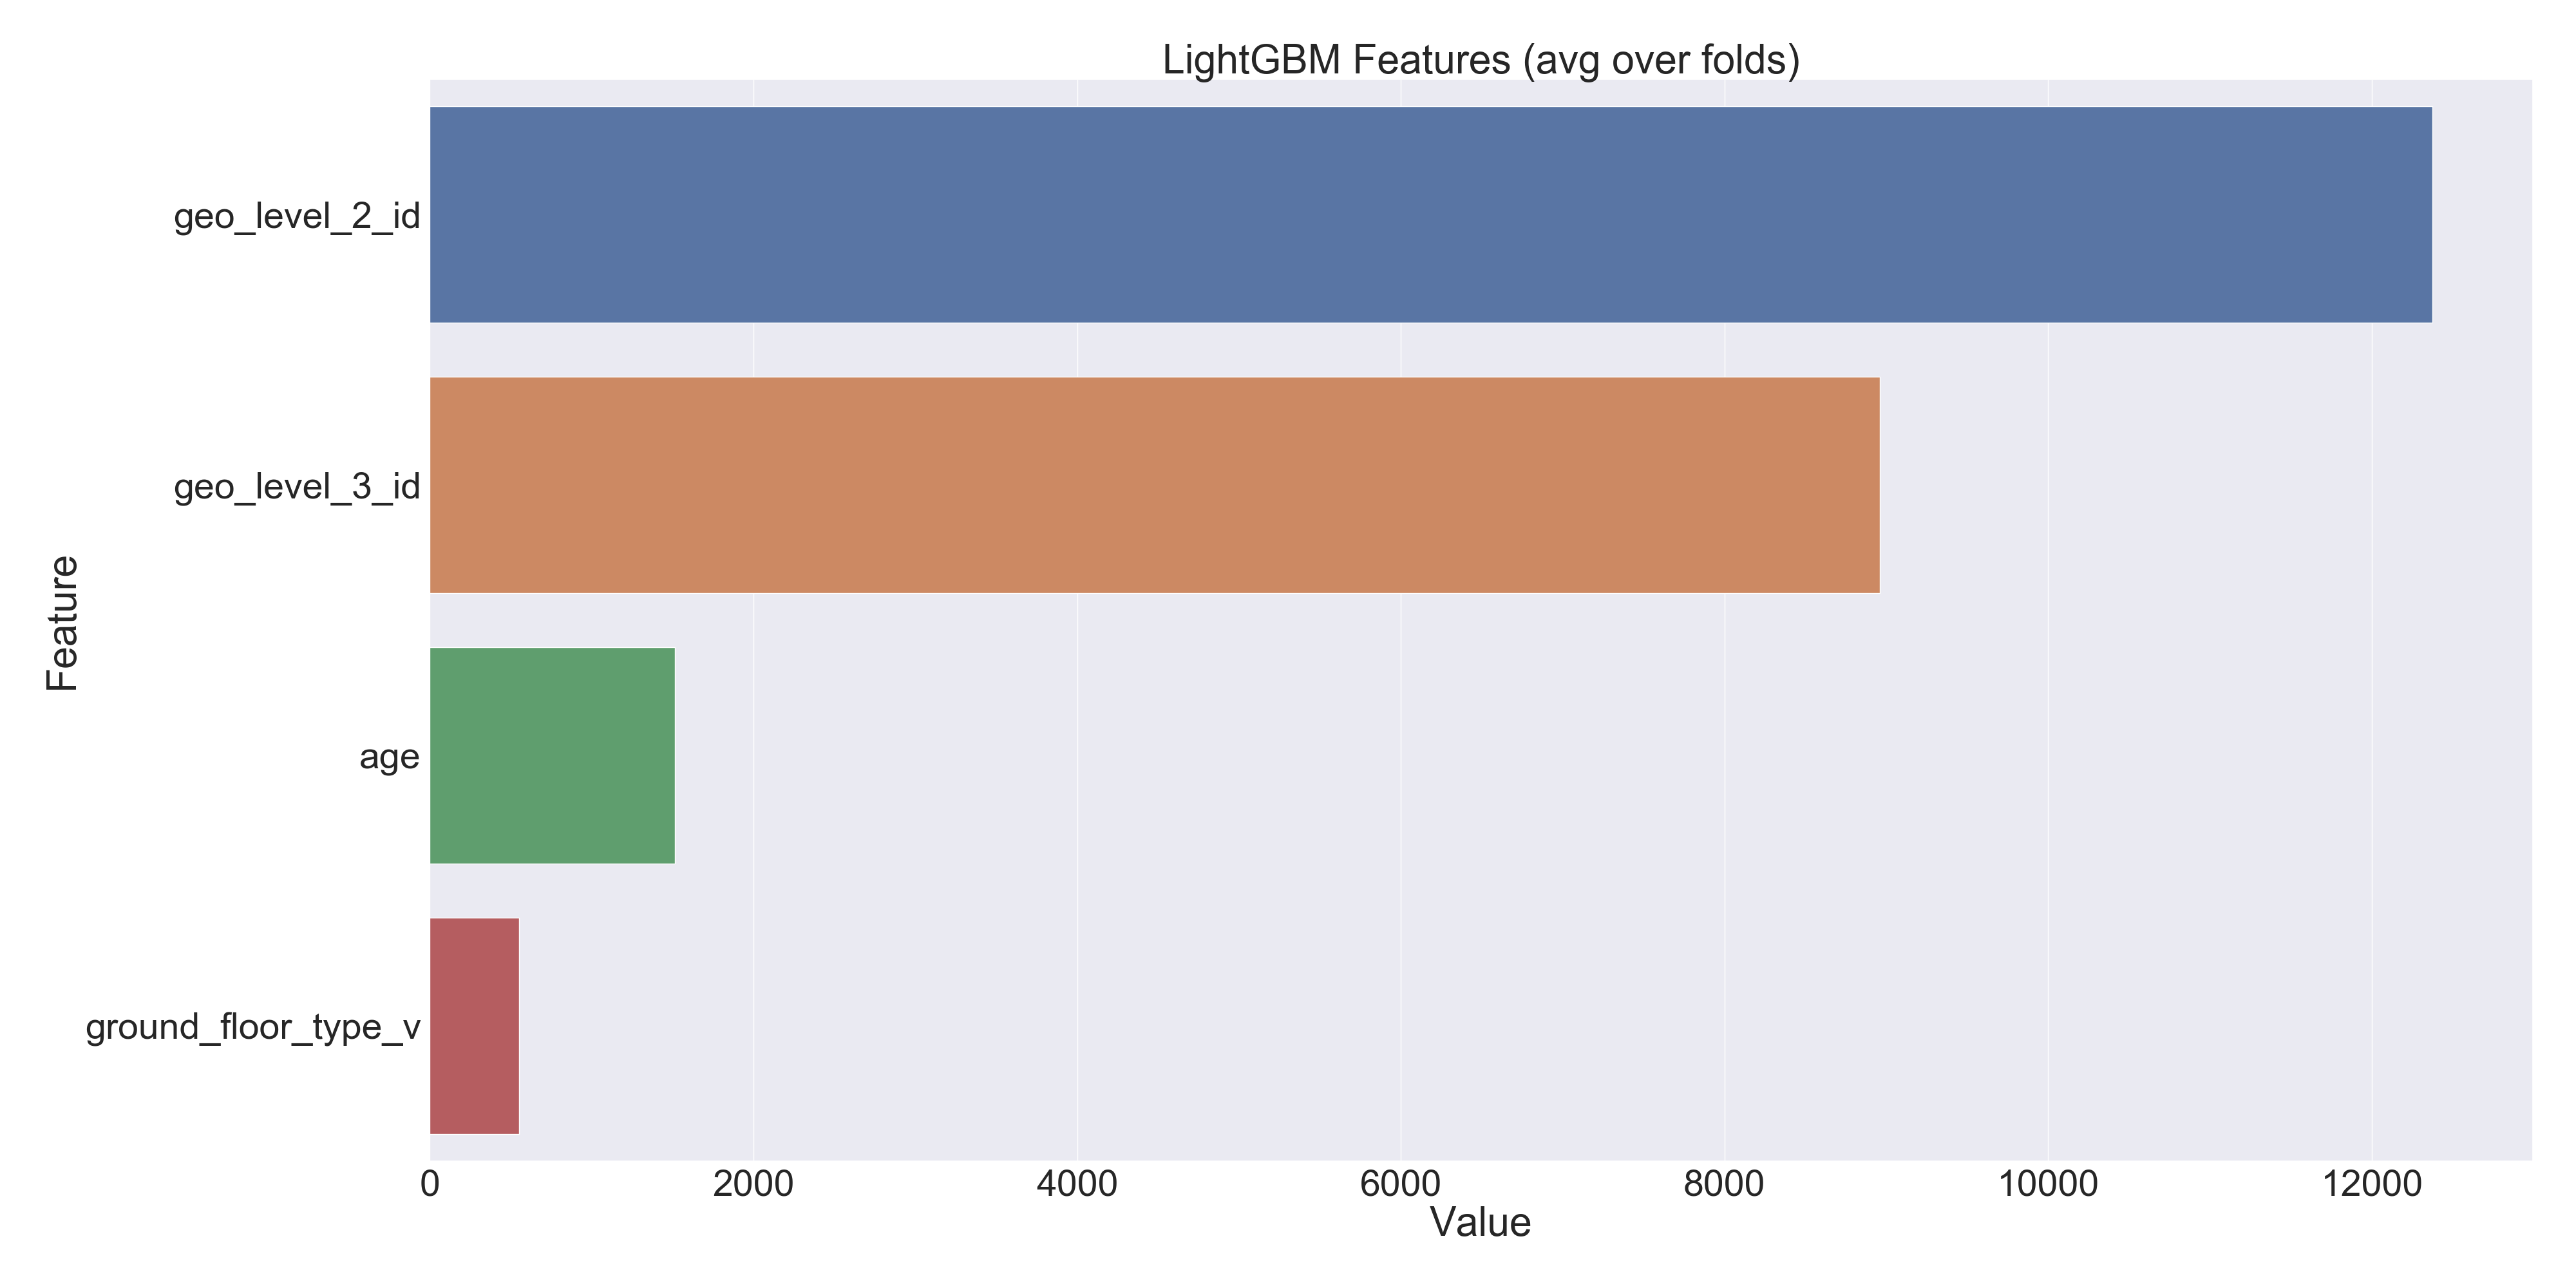
\includegraphics[height=0.9\textwidth, width=1.0\textwidth]{lgbm_importances_05_10}
    \caption{Importancia de las variables tras seleccionar las 10 mejores. }
    \label{fig:lgbm_imp_05_10}
\end{figure}

Si nos quedamos solo con 4 variables no selecciona estas cuatro y el rendimiento baja a 0.6772.

Como no sabemos cuál es la mejor forma de seleccionar el valor $k$ del preprocesado realizamos pruebas con algunos valores para elegir el mejor. En la Tabla \label{tab:05_k} podemos ver los diferentes valores probados.

\begin{table}[H]
\centering
\caption{Selección de las $k$ mejores características.}
\label{tab:05_k}
\begin{tabular}{lrr}
\toprule
Nº de variables & F1-Score & Tiempo por partición ($s$)\\
\midrule
4 & 0.6772 & ~7\\
10 & 0.7251 & 9.5 - 13\\
20 & 0.7296 & 10 - 15\\
25 & 0.7317 & 12 - 17\\
30 & 0.7325 & 17 - 18\\
35 & 0.7335 & 18 - 20\\
37 & 0.7294 & 19 - 21\\
40 & 0.7302 & 18 - 23\\
\bottomrule
\end{tabular}
\end{table}

Nos quedamos con 35 variables... consiguiendo una puntuación en test de 0.7228 (parecida a la conseguida sin realizar la selección de variables). En la Figura \label{fig:lgbm_imp_05_35} observamos las variables más utilizadas para clasificar.

\begin{figure}[H]
    \centering
    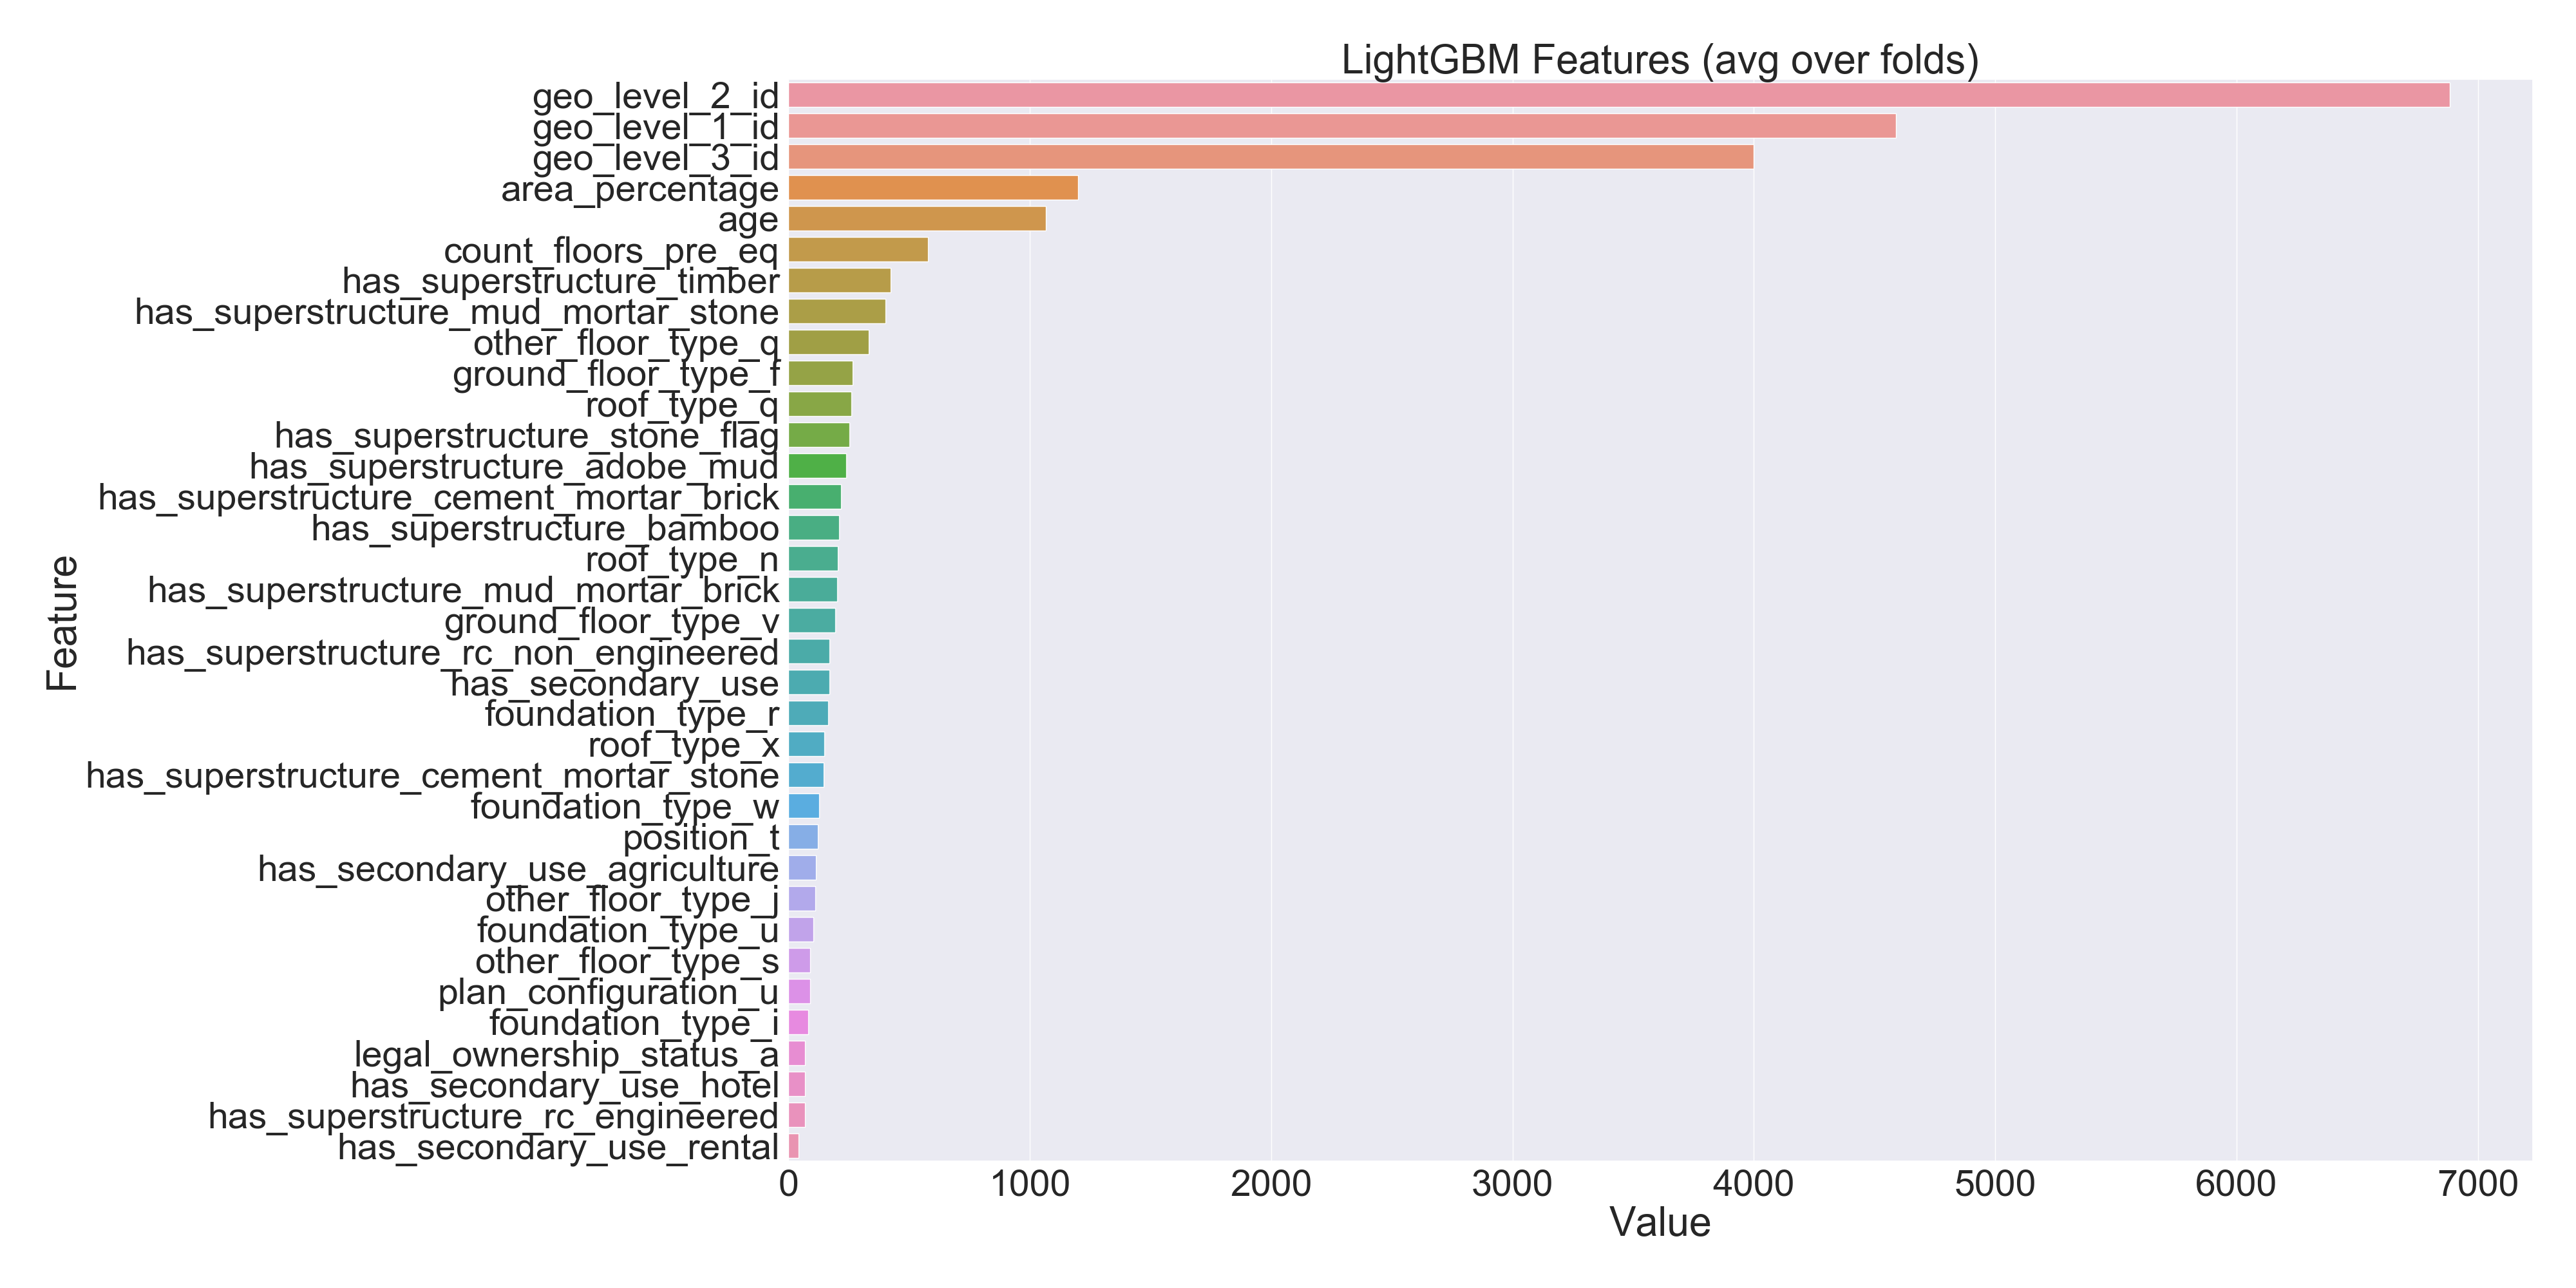
\includegraphics[height=0.9\textwidth, width=1.0\textwidth]{lgbm_importances_05}
    \caption{Importancia de las variables tras seleccionar las 35 mejores. }
    \label{fig:lgbm_imp_05_35}
\end{figure}

Comparando con las seleccionadas en p3\_04 nos damos cuenta de que aunque las primeras son similares y coinciden en algunas más, \texttt{height\_percentage} es de las más utilizadas en el caso anterior y en este no fue seleccionada.

\subsection{\texttt{p3\_06}}
Tras perder el rato con algunas pruebas fallidas, decido no desperdiciar la última subida del día tratando de mejorar aumentando el número de hojas a 45. Puntuación en training: 0.7375, puntuación en test: 0.7253.


\subsection{Pruebas fallidas}
%https://lightgbm.readthedocs.io/en/latest/Parameters.html#categorical_feature
Tras observar los parámetros de Lightgbm nos damos cuenta de que tiene una opción en la que el propio algoritmo trata este tipo de variables. Probamos a usar esta opción para comparar con el rendimiento que obtuvimos en \texttt{p3\_00}.
 No funciona (p3\_categorical.py)
 ValueError: could not convert string to float: 't'
\subsubsection{umap}
% https://umap-learn.readthedocs.io/en/latest/
Por recomendación de un compañero, pruebo a utilizar umap para reducir la dimensionalidad. Tras instalar el paquete mediante \texttt{pip install umap-learn}, pruebo su funcionamiento de forma básica en \texttt{p3\_umap.py} (algoritmo: lightgbm).

Tras largo tiempo de ejecución (media hora por lo menos) consigue exactamente los mismos resultados que p3\_00 :( (resultados en submissions\_ap.csv)
\subsubsection{Información mutua}
Tras p3\_04...

Probamos a utilizar como criterio la información mutua, que representa el grado de dependencia entre dos variables, la información que una contiene sobre la otra. Si vale 0 es porque las variables son independientes... p3\_mi.py
notamos que tarda mucho, puede ser porque se basa en cosas tipo knn que con el alto número de instancias es excesivamente lento...

\subsubsection{Boruta}
Para terminar los experimentos de selección de variables con Lightgbm utilizaremos Boruta, que pretende seleccionar las variables más importantes sin que tengamos que fijar de antemano el número de variables a utilizar.

Partiendo del código proporcionado por el profesor de prácticas utilizaremos un RandomForest para seleccionar las características más importantes. Nuestra primera impresión es negativa debido al alto tiempo de cómputo 142.44 segundos para seleccionar.

Tarda del orden de 2700 segundos y me da un error :/ mala idea un random forest con tantas variables.

% TODO:
% - Pasar a textit: script, test, training, boosting
% TODO:
% - Referenciar referencias...
%%%%%%%%%%%%%%%%%%%%%%%%%%%%%%%%%%%%%%%%%%%%%%%%%%%%%%%%%%%%%%%%%%%
%       REFERENCIAS
%%%%%%%%%%%%%%%%%%%%%%%%%%%%%%%%%%%%%%%%%%%%%%%%%%%%%%%%%%%%%%%%%%%
\printbibliography
\end{document}
